\subsection{(111)-Goldschicht}
Die Rauheit der Goldschicht sollte mit dem RTM bestimmt werden. Dazu wurde die Oberfl�che der Goldschicht mit dem RTM im CC-Mode abgerastert.
Wegen der Kornstruktur wurden f�r die Bestimmung der Fl�chenrauheit zwei Messungen vorgenommen, sodass Korngrenzen nur in der ersten Messung in die Berechnung der Rauheit eingingen. Die (111)-Goldschicht musste aufgrund von Kratzern auf der Oberfl�che mehrfach gedreht werden. W�hrend der Justierung ist die Pt-Ir-Spitze des RTM mit der Oberfl�che der Goldschicht kollidiert, sodass eine zweite Pt-Ir-Spitze angefertigt werden musste. Diese konnte ebenfalls nach wenigen Versuchen aus bereits benutzten Pt-Ir-Spitzen angefertigt werden.
\subsubsection{Rauheit}
\begin{figure}[H]
\centering
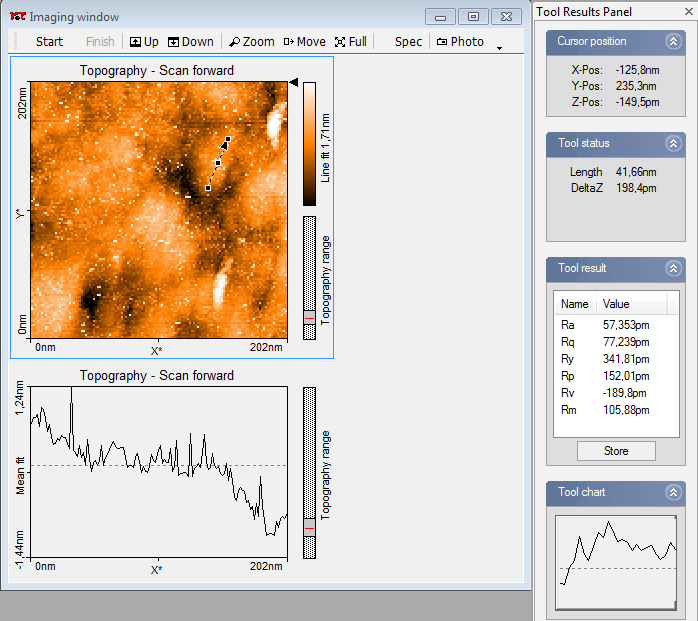
\includegraphics[scale = 0.75]{Gold_linienrauheit_202nm}
\caption{ Mittlere Linienrauheit der (111)-Goldschicht ($R_a = \SI{57,353}{pm}$ und $R_q = \SI{77,239}{pm}$) }
\end{figure}
\begin{figure}[H]
\begin{subfigure}[t]{0.49\textwidth}
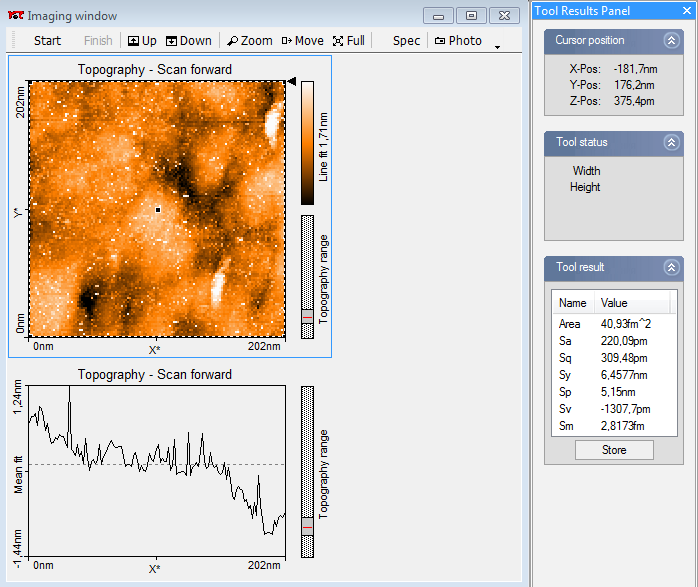
\includegraphics[scale = 0.45]{Gold_flaechenrauheit_202nm_2}
\caption{Mittelung �ber die gesamte Fl�che, da durch die Kornstruktur keine gro�e glatte Fl�che zu finden war. ($S_a = \SI{220,09}{pm}$ und $S_q = \SI{309,48}{pm}$)}
\end{subfigure}
\hspace{0.02\textwidth}
\begin{subfigure}[t]{0.49\textwidth}
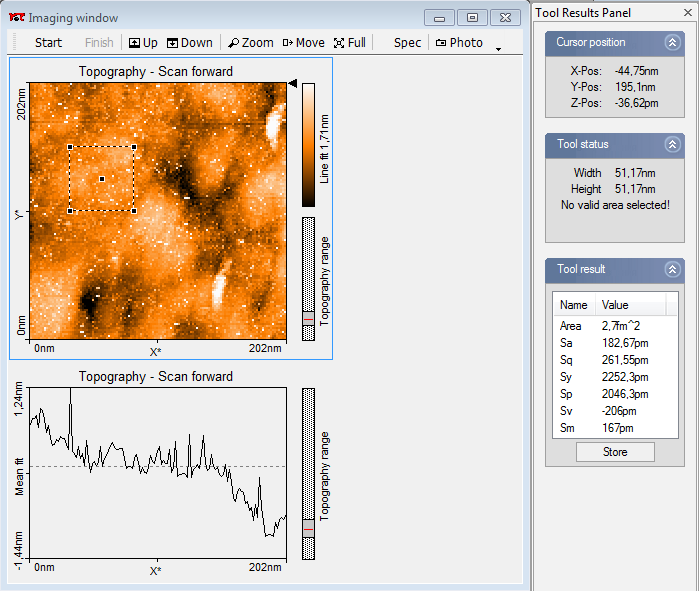
\includegraphics[scale = 0.45]{Gold_flaechenrauheit_202nm_1}
\caption{Mittelung eine kleinere m�glichst glatte Fl�che. Die Verkippung wurde bei allen Messungen korrigiert. ($S_a = \SI{182,67}{pm}$ und $S_q = \SI{261,55}{pm}$)}
\end{subfigure}
\caption{ Mittlere Fl�chenrauheit der (111)-Goldschicht}
\end{figure}
\subsubsection{Monoatomare Stufen und Gitterdefekte}